\documentclass[a4paper,12pt]{article}

% Use the graphicx package for image inclusion
\usepackage{graphicx}

% Page setup
\usepackage{geometry}
\geometry{top=2.5cm, bottom=2.5cm, left=2.5cm, right=2.5cm}

% Title and author setup
\title{\vspace{-4cm}Seminarska naloga za Računalniško grafiko\\[0.5cm] \huge \textbf{Frodo's Nightmares} \vspace{-1cm}}
\author{}
\date{}

\begin{document}

\begin{titlepage}
    \begin{center}
        \vspace*{2cm}

        \textbf{\Huge{Seminarska naloga za Ra\v{c}unalni\v{s}ko grafiko}}

        \vspace{0.5cm}

        \textbf{\LARGE{Frodo's Nightmares}}

        \vfill

        \hspace*{-1.5cm} Mentor: izr. prof. dr. Iztok Lebar Bajec
        \hspace*{2.5cm} Ljubljana, januar 2025
        \hspace*{2cm} Tim Thuma, 63230333, Luka Hribar, 63230109, Tilen Medved, 
    \end{center}
\end{titlepage}

% Abstract section
\section*{\textit{Abstract}}

\noindent Here you can write the abstract of your work. This should give a concise summary of your research, game design, and findings.

\newpage

% Pregled igre section
\section{Pregled igre}

\subsection{Opis sveta}
\noindent This section contains the description of the game world.

\subsection{Pregled}
\noindent Here you can describe an overview of the game.

\subsection{Ozadje}
\noindent This is the background of the game. You can insert an image here:

\begin{figure}[h!]
    \centering
    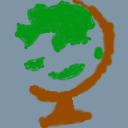
\includegraphics[width=0.5\textwidth]{./slika.png}
\end{figure}

\subsection{Ključne lokacije}
\noindent Describe the key locations within the game world here.

\subsection{Velikost}
\noindent Discuss the size of the game world or levels.

\subsection{Objekti}
\noindent Describe the main objects or elements in the game.

\newpage

% Igralni pogon section
\section{Igralni pogon}
\noindent This section describes the game engine used, its features, and how it supports the gameplay.

\newpage

% Pogled section
\section{Pogled}
\noindent This section describes the perspective or camera view in the game.

\newpage

% Osebek section
\section{Osebek}
\noindent Here you describe the protagonist or main character of the game.

\newpage

% Uporabniški vmesnik section
\section{Uporabniški vmesnik}
\noindent This section describes the user interface of the game, how the user interacts with it, and any menus or controls.

\newpage

% Gameplay section
\section{Gameplay}
\noindent Here you can describe the gameplay mechanics, objectives, challenges, and how players interact with the game world.

\newpage

% Zaključki in možne nadgradnje section
\section{Zaključki in možne nadgradnje}
\noindent Conclude your work here, and suggest possible improvements or upgrades for the game.

\end{document}
